\documentclass{fizykalab}

% Ustawienia do tabelki

\wydzial{WI}
\autorjeden{Dawid Komęza}
\autordwa{Magdalena Śmietana}
\rok{II}
\grupa{14}
\zespol{2}
\temat{Kriogenika}
\nrcwiczenia{113}
\datawykonania{07.11.2025}
\dataoddaniajeden{14.11.2025}
\zwrotdopoprawy{}
\dataoddaniadwa{}
\datazaliczenia{}

\begin{document}

\maketitle

\section{Cel ćwiczenia}
Celem ćwiczenia jest zapoznanie z urządzeniami
kriogenicznymi wykorzystującymi ciekły azot oraz
badanie właściwości cieplnych azotu. W szczególności zależność temperatury wrzenia od ciśnienia,
pomiar parametrów punktu potrójnego oraz wartość ciepła parowania azotu.

\begin{figure}[h!]
    \centering
    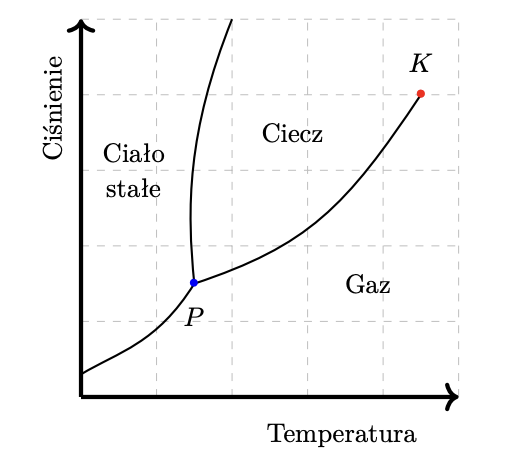
\includegraphics[width=0.7\textwidth]{triple_critical_point.png}
    \caption{Punkt potrójny (P) oraz punkt krytyczny (K) widoczne na wykresie ciśnienia od temperatury}
    \label{fig:triple_critical_point}
\end{figure}

\section{Wstęp teoretyczny}
Kriogenika to dziedzina nauki i techniki zajmująca się badaniem i wykorzystaniem niskich temperatur. Powszechnie używaną cieczą kriogeniczną
jest ciekły azot o temperaturze wrzenia 77 K oraz
temperaturze topnienia 63.1 K (pod ciśnieniem atmosferycznym). Wraz ze wzrostem ciśnienia wzrasta temperatura wrzenia, aż do osiągnięcia punktu
krytycznego K, natomiast wraz ze zmniejszaniem
się ciśnienia maleje temperatura wrzenia, aż do osiągnięcia punktu potrójnego P (Rysunek 1) którego
właściwości będziemy badać. W ramach ćwiczenia będziemy musieli wyznaczyć ciepło parowania azotu.
Z definicji jest to ilość energii potrzebnej do odparowania jednostki masy danej substancji przy stałym
ciśnieniu i temperaturze. Będziemy je wyznaczać używając układu równań złożonego z równań bilansu
cieplnego dla strat cieplnych bez grzejnika oraz z grzejnikiem.

\section{Aparatura pomiaru}
Podczas przeprowadzania doświadczenia będziemy korzystać z naczyń Dewara. Naczynie to jest przystosowane do przechowywania cieczy o niskiej temperaturze wrzenia. Swoje właściwości zawdzięcza podwójnej ściance z próżnią, która zapobiega przewodnictwu cieplnemu i konwekcji. Nie zapobiega jednak
przed promieniowaniem cieplnym oraz przewodzeniem ciepła przez połączenie ścianki wewnętrznej z
zewnętrzną.
Do pierwszej części ćwiczenia wykorzystamy kriostat wyposażony w: manometr mechaniczny (wyznaczający różnicę między ciśnieniem atmosferycznym a ciśnieniem w kriostacie), opornik platynowy wraz
z omomierzem (wykorzystujący zależność rezystancji od temperatury przewodnika – wraz ze wzrostem
temperatury rezystancja rośnie) oraz połączenie z pompą próżniową.

\begin{figure}[h!]
    \centering
    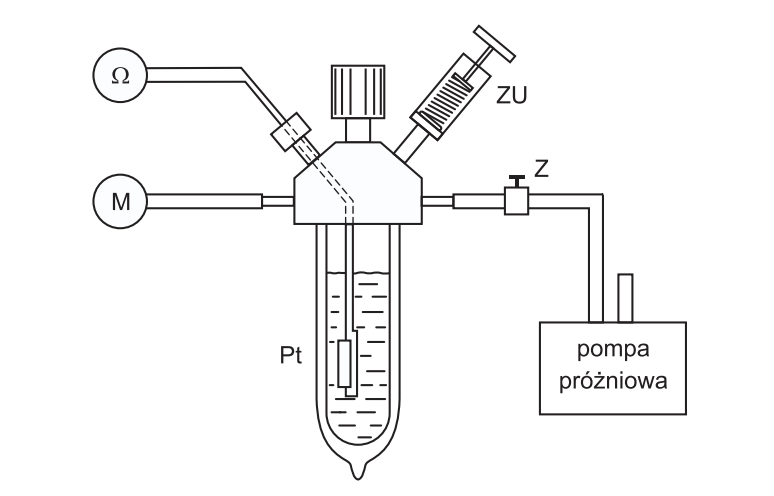
\includegraphics[width=0.7\textwidth]{pompa_prozniowa.png}
    \caption{Układ pomiarowy do wyznaczania zależności temperatury wrzenia azotu od ciśnienia i do uzyskiwania zestalonego azotu }
    \label{fig:pomba_prozniowa}
\end{figure}

\section*{Wzory}

\begin{enumerate}
    \item \textbf{Bilans cieplny bez dodatkowego źródła ciepła:}
    \begin{equation}
        P_s \, t_1 = \Delta m_1 \, Q_p
        \label{eq:bilans1}
    \end{equation}

    \item \textbf{Bilans cieplny z dodatkową mocą grzejnika:}
    \begin{equation}
        (P_s + P) \, t_2 = \Delta m_2 \, Q_p
        \label{eq:bilans2}
    \end{equation}
    gdzie:
    \begin{itemize}
        \item $P_s$ – moc strat cieplnych kriostatu,
        \item $P = U I$ – moc doprowadzona przez grzejnik,
        \item $t_1, t_2$ – czasy odparowania masy $\Delta m$ bez i z grzejnikiem,
        \item $Q_p$ – ciepło parowania.
    \end{itemize}

    \item \textbf{Równanie Clausiusa–Clapeyrona:}
    \begin{equation}
        \frac{dT}{dp} = \frac{T \, (V_2 - V_1)}{Q}
        \label{eq:clausius_clapeyron}
    \end{equation}
    lub równoważnie:
    \begin{equation}
        Q = T \, (V_2 - V_1) \, \frac{dp}{dT}
    \end{equation}
    gdzie:
    \begin{itemize}
        \item $Q$ – ciepło przemiany (np. parowania),
        \item $T$ – temperatura przemiany,
        \item $V_2 - V_1$ – różnica objętości właściwych faz (gazowej i ciekłej),
        \item $\frac{dT}{dp}$ – pochodna temperatury wrzenia względem ciśnienia.
    \end{itemize}

    \item \textbf{Równanie gazu doskonałego (dla obliczenia objętości właściwej azotu gazowego):}
    \begin{equation}
        pV = nRT
        \label{eq:ideal_gas}
    \end{equation}
    stąd objętość właściwa gazu:
    \begin{equation}
        V_g = \frac{RT}{M p}
        \label{eq:v_specific}
    \end{equation}
    gdzie:
    \begin{itemize}
        \item $R$ – stała gazowa,
        \item $M$ – masa molowa azotu,
        \item $p$ – ciśnienie,
        \item $T$ – temperatura gazu.
    \end{itemize}

    \item \textbf{Zależność ciepła przemiany z równania Clausiusa–Clapeyrona dla cieczy i gazu:}
    \begin{equation}
        Q_p = T \, (V_g - V_c) \, \frac{dp}{dT}
    \end{equation}

    \item \textbf{Moc cieplna opornika:}
    \begin{equation}
        P = U I
        \label{eq:power}
    \end{equation}

\end{enumerate}

\section{Wykonanie}
\subsection{Wyzanczenie zależności temperatury wrzenia od ciśnienia oraz punktu
potrójnego}
Po ochłodzeniu naczynia Dewara napełniliśmy je ciekłym azotem oraz wykonaliśmy pomiar temperatury
poprzez odczytanie wartości oporu oraz wykorzystanie
podanej zależności temperatury od oporu. Opór przy
ciśnieniu atmosferycznym wynosił XX Ω, czyli temperatura wynosiła XX K. Zgodnie z treścią doświadczenia
zaczęliśmy od zwiększania ciśnienia, na skutek wrzenia
azotu, który w formie gazowej zajmuje większą objętość. Następnie poprzez wykorzystanie pompy próżniowej zmniejszaliśmy ciśnienie aż do punktu potrójnego,
czyli momentu, w którym azot jednocześnie wrzał oraz
krzepnął. Trzy razy wyznaczając współrzędne punktu
potrójnego otrzymaliśmy te same wyniki, mianowicie
ciśnienie równe XX bar oraz opór XX Ω (czyli temperatura XX K). Dane zgromadzone podczas pomiaru wraz
z temperaturami znajdują się w tabeli.



\subsection{Pomiar ciepła parowania}
Po ochłodzeniu naczynia Dewara, napełniamy to naczynie do ustalonej wysokości (14 cm na podziałce)
oraz mierzymy czas, w którym wysokość zmniejszy się o 6 cm (do wys. 8 cm na podziałce). Powtarzamy
doświadczenie przy włączonym grzejniku. Na skutek przepływu prądu przez opornik, wytwarza się ciepło,
które wpływa na szybkość procesu wrzenia azotu. Czas parowania z wyłączonym grzejnikiem wyniósł
XX, oraz z włączonym XX. Zmierzona średnica przekroju naczynia wynosiła d = XX cm

\section{Wnioski}

\end{document}
